\section{Pendule à $N$ maillons}

\renewcommand*{\overrightarrow}[1]{\vbox{\halign{##\cr 
  \tiny\rightarrowfill\cr\noalign{\nointerlineskip\vskip1pt} 
  $#1\mskip2mu$\cr}}}

Dans cette partie, nous allons considérer deux types de pendules à n maillons (le pendule simple et le pendule double) et chercher à 
résoudre leur équation du mouvement par les méthodes numériques implémentées dans la première partie.

\subsection*{Le pendule simple} Dans le cas du pendule simple, il y a deux forces qui s'appliquent sur la masse $ m $: le poids de la masse \overrightarrow{P} et la force de la tige \overrightarrow{T}.
D'après le théorème du moment cinétique appliqué en M par rapport à O on a
\begin{equation}
  \frac{d\overrightarrow{L_{O,M}}}{dt} = \overrightarrow{M_{O, M}(\overrightarrow{P})} + \overrightarrow{M_{O, M}(\overrightarrow{T})} \nonumber
\end{equation}

Le moment de \overrightarrow{T} est nul car \overrightarrow{OM} et \overrightarrow{T} sont colinéaires. En développant l'expression, on a alors 
$ m l^{2} \ddot \theta = - m l g \sin{\theta} $, ce qui nous donne finalement 
\begin{equation}
	\ddot \theta + \frac{g}{l} \sin{\theta}= 0 \nonumber
\end{equation}

On retrouve l'équation différentielle non linéaire du second ordre bien connu du pendule simple. 
Pour la résoudre numériquement en fonction de l'angle initial $ \theta_{0} $, on peut utiliser une des méthodes 
implémentées dans la première partie comme par exemple la méthode d'Euler.

Une fois trouvée la fonction $ \theta(t) $, on peut calculer la période du pendule en prenant la différence entre 
deux maximum successifs. Pour enfin déterminer la fréquence.

\bigskip

En affichant les différentes fréquences du pendule pour des valeurs de $ \theta_{0} $ variant de $ -\frac{\pi}{2} $ à $ \frac{\pi}{2} $, 
on obtient la figure~\ref{fig:frequences} suivante:

\begin{figure}[htbp!]
	\centering
	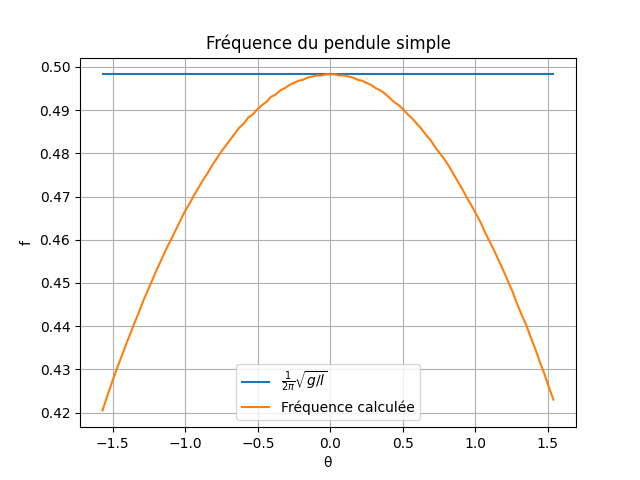
\includegraphics[width=0.5\textwidth]{res/freq_pendule_simple.png}
	\caption{Fréquence du pendule en fonction de l'angle initial $ \theta_{0}$}
	\label{fig:frequences}
\end{figure}

\bigskip

On remarque bien que pour des valeurs de $ \theta_{0} $ faible représentant les petites oscillations du pendule, 
la fréquence est égale à la valeur $ \frac{1}{2 \pi} \sqrt{\frac{g}{l}} $.

\subsection*{Le pendule double} Le pendule à deux maillons est constitué de deux masse $ m_{1} $ et $ m_{2} $ 
reliées par deux tiges de longueur $ l_{1} $ et $ l _{2} $. On note $ \theta_{1} $ et $ \theta_{2} $ les angles
que font les tiges avec la verticale. On a alors les deux équations suivantes qui décrivent le mouvement du pendule:
\begin{equation}
	\begin{cases}
		\ddot \theta_{1} = \frac{m_{2} g \sin(\theta_{2}) \cos(\theta_{1} - \theta_{2}) + m_{2} l_{1} \dot \theta_{1}^{2} \sin(\theta_{1} - \theta_{2}) \cos(\theta_{1} - \theta_{2}) + m_{2} l_{2} \dot \theta_{2}^{2} \sin(\theta_{1} - \theta_{2}) - (m_{1} + m_{2}) g \sin(\theta_{1})}{(m_{1} + m_{2}) l_{1} - m_{2} l_{1} \cos^{2}(\theta_{1} - \theta_{2})}  \\ \nonumber
		\ddot \theta_{2} = \frac{- m_{2} l_{2} \dot \theta_{2}^{2} \sin(\theta_{1} - \theta_{2}) \cos(\theta_{1} - \theta_{2}) + (m_{1} + m_{2}) (g \sin(\theta_{1}) \cos( \cos(\theta_{1} - \theta_{2})) - l_{1} \dot \theta_{1}^{2} \sin(\theta_{1} - \theta_{2}) - g \sin(\theta_{2}))}{(m_{1} + m_{2}) l_{2} - m_{2} l_{2} \cos^{2}(\theta_{1} - \theta_{2})}  
	\end{cases}
	\label{eq:pendule_2_maillons}
\end{equation}

Ce sont deux équations différentielles non linéaires du second ordre. 
On peut résoudre numériquement ce système d'équations différentielles couplées en utilisant la méthode de Runge-Kutta d'ordre 4.

\bigskip

En dessinant les trajectoires des pendules pour deux conditions initiales différentes mais très proches comme par exemple 
$ \theta_{1}(0) = \frac{\pi}{2} $, $ \dot \theta_{1}(0) = \dot \theta_{2}(0) = 0 $, avec seulement une différence sur l'angle initial $ \theta_{2}(0) $ de 12 degré (soit $ \theta_{2}(0) = 0 $ et $ \theta_{2}(0) = \frac{\pi}{15} $),
on obtient les figures~\ref{fig:traj_0} et~\ref{fig:traj_12} suivante:

\begin{figure} [htbp!]
  \begin{minipage}[c]{0.5\textwidth}
	\centering
	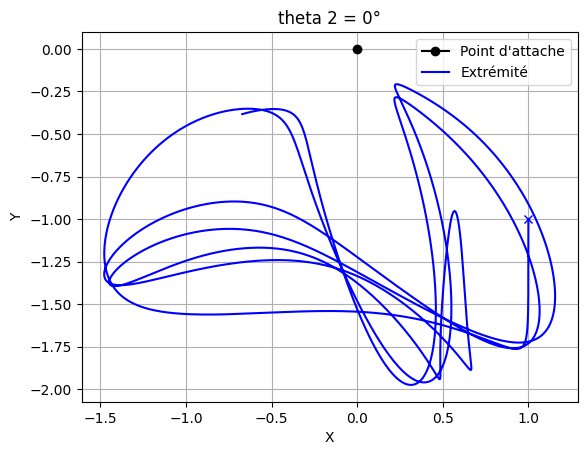
\includegraphics[width=\textwidth]{res/traj_0.png}
	\caption{Trajectoire pour $ \theta_{2}(0) = 0 $}
	  \label{fig:traj_0}
  \end{minipage}\hfill
  \begin{minipage}[c]{0.5\textwidth}
	\centering
	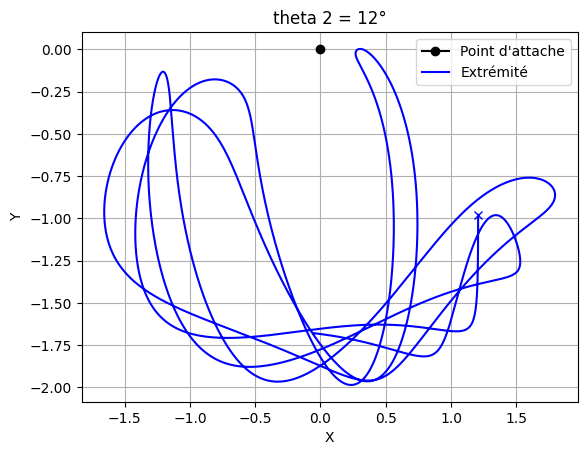
\includegraphics[width=\textwidth]{res/traj_12.png}
	\caption{Trajectoire pour $ \theta_{2}(0) = \frac{\pi}{15} $}
	  \label{fig:traj_12}
  \end{minipage}
\end{figure}

Les croix représentent le début du parcours de l'extrémité de chaque pendule et on remarque que les trajectoires suivent tout d'abord le même chemin puis divergent complètement au fur et à mesure que le temps avance.

À l'inverse du pendule simple où les trajectoires sont des ellipses peut importe les conditions initiales, 
le pendule double est quant à lui un système très sensible à celles-ci: c'est un système chaotique.  

\bigskip

Une fois les trajectoires calculées, on peut s'intéresser au temps que met le pendule à se retourner (la masse $ m_{2} $ passe au
dessus de $ m_{1} $).
Ce retournement arrive lorsque $ \theta_{2} $ dépasse en valeur absolue $ \pi $.
Pour des conditions initiales bien choisies, on peut observer un pendule qui ne se retourne jamais. Comme par 
exemple avec des conditions initiales proche de zéro comme on peut le voir sur la figure~\ref{fig:no_retournement}. 

Mais si on vient à augmenter les valeurs des angles initiaux, ou 
des vitesses angulaires initiales, on peut observer un retournement du pendule. Comme par exemple avec les conditions initiales suivantes:
$ \dot \theta_{1} = 8 $ rad/s et des valeurs nulles pour les autres paramètres. On obtient alors la figure~\ref{fig:retournement} dans laquelle on peut observer le retournement du pendule.
on peut observer le retournement du pendule (au bout de 5.3 secondes).

\begin{figure} [htbp!]
	\begin{minipage}[c]{0.5\textwidth}
		\centering
		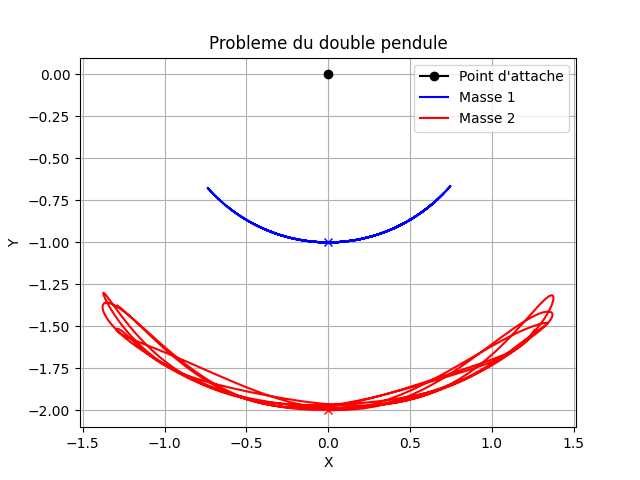
\includegraphics[width=\textwidth]{res/no_retournement.png}
		\caption{Pas de retournement du pendule}
		\label{fig:no_retournement}
	\end{minipage}\hfill
	\begin{minipage}[c]{0.5\textwidth}
		\centering
		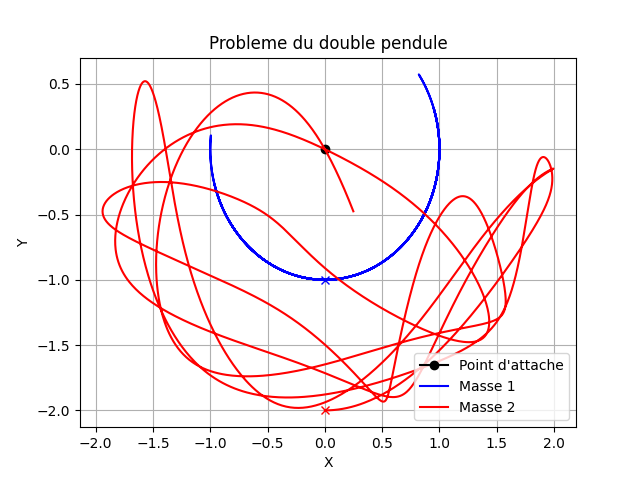
\includegraphics[width=\textwidth]{res/retournement.png}
		\caption{Retournement du pendule}
		\label{fig:retournement}
	\end{minipage}
\end{figure}
